\part{Towards Highly Miniaturized LED Power Systems }
\label{ch:twrd_HMLED}

\chapter[LEDification]{LEDification: The second lighting revolution}


The light bulb was one of the most relevant inventions form our past history.  Electrical lighting was definitely a revolution in the early 19$^{th}$ century society; for the first time in the history, human kinds had a clear, reliable and safe source of artificial light that was easy to distribute and control.
The apparition  of the electrical light bulb was also, with no doubt, the trigger for the commercialization of electric power and the deployment of the first power distribution networks. The impact was to such degree that it settled two of capital sectors from the present industry, the lighting and the electric power distribution, with  world recognized companies such as Philips, General Electric or Osram.  Actually, both sectors have been so close related that even often we use the word \emph{light} when we actually are refereing electricity. In resume, a single invention changed our society for ever, bringing light and electricity to our homes.

\begin{figure}[!h]
\centering
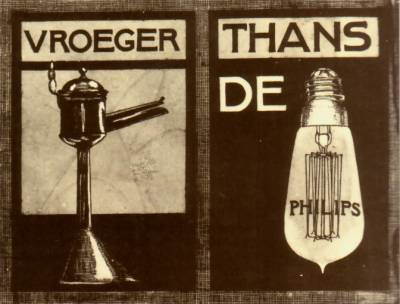
\includegraphics{./0_intro/img/1900-philips3.jpg}
\caption{Early incandescent light bulb}
\label{fig:incandescent_light_blub}
\end{figure}


From the initial invention of the first incandescent light bulb,  bulbs have just been illuminating our daily lives without having  any \emph{enlightening} relevance or sense of innovation. Despite our impression,  important research has continuously been done to improve the worst characteristic of the incandescent light bulb, the efficacy. Incandescent light bulbs are extremely inefficient to generate light with a luminous efficacy between $12.6 lm/W$, for a tungsten incandescent bulb, up to $24 lm/W$ for a quartz halogen bulb (see Table~\ref{tab:lighting_tech}). In a more comprehensive way, we can say that in general incandescent lights convert at least 95\% of the supplied power in heat and just, at most 5\% in light. Knowing that lighting represents 17\% of world energy consumption, we can account that 15\% of the world consumed power is transformed in to heat and only a 1.7\% is transformed in real light \footnote{Estimated 2008 values}. Therefore these figures illustrate  the motivation and necessity of improving the efficacy of the light bulbs.

\begin{figure}[!h]
\centering
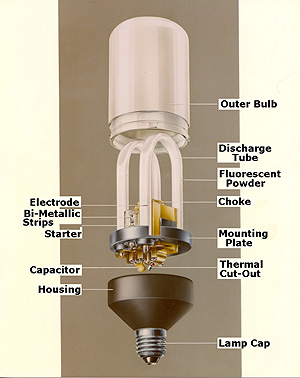
\includegraphics{./0_intro/img/phil1b.jpg}
\caption{Components of the Philips SL compact fluorescent lamp. }
\label{fig:philips_sl}
\end{figure}

Gas-discharge lamps where the first alternative of the incandescent lamps benefiting with a better efficacy, being the fluorescent tub the most popular among the family. The low pressure mercury-vapor gas-discharge  lamp, florescent tube, could be considered an innovation in the lighting. Initial the tubs where mainly used for big spaces warehouses, factories and offices, and later one, in the late 80's, started populating domestic houses with the appearance of the \emph{compact fluorescent lamps}\footnote{Screw-in version of a fluorescent tube. Now a days you can find a CFL replacement for almost the majority of sockets in the market.} (CFLs), being now a days the market standard for energy efficient light bulbs, shown in Figure~\ref{fig:philips_sl}. Florescent lamps are indeed a big improvement in efficacy with respect to the incandescent lamps. The luminous efficacy ranges between 52-100 $lm/W$, depending on the light color temperature, converting about 22\% of the input power to visible light, more details of other gas-discharge bulbs is presented in Table~\ref{tab:lighting_tech}. Although the better efficiency of the CPL they did not fully replace the inefficient incandescent ones due to the following reasons~\cite{11EPA}:
\begin{itemize}
  \item Standard CFLs are not \emph{dimmable}.  \emph{Simmable} CFLs are more expensive, their behaviour is not standardized among manufacturers and does not match the consumers desires.
  \item CFLs have a slow warm-up time\footnote{Gas-discharge lamps has to be warm in order to volatilise and mix chemical elements that compose the gas. Depending on the element that can take from few minutes up to tens of minutes. }. Not being suitable for places where lights are turned on for short times.
  \item CFLs have different form and look. Some ones can not fit in some fixtures that mount incandescent lamps. The \emph{pig tail} appearance is not attractive when bulbs are exposed.
  \item The small prices of the incandescent light bulbs compared to CFLs are more attractive for the consumer. Although CFLs save more money due to power savings, the end consumers are still biased by the retail price of the lamps.
\end{itemize}
Therefore in 2012 was estimated that still more than 50\% of the installed light bulbs where still incandescent in residential environments. Thus still a need for a lighting technology capable of replacing the old inefficient incandescent lamps.

\begin{figure}[!h]
\centering
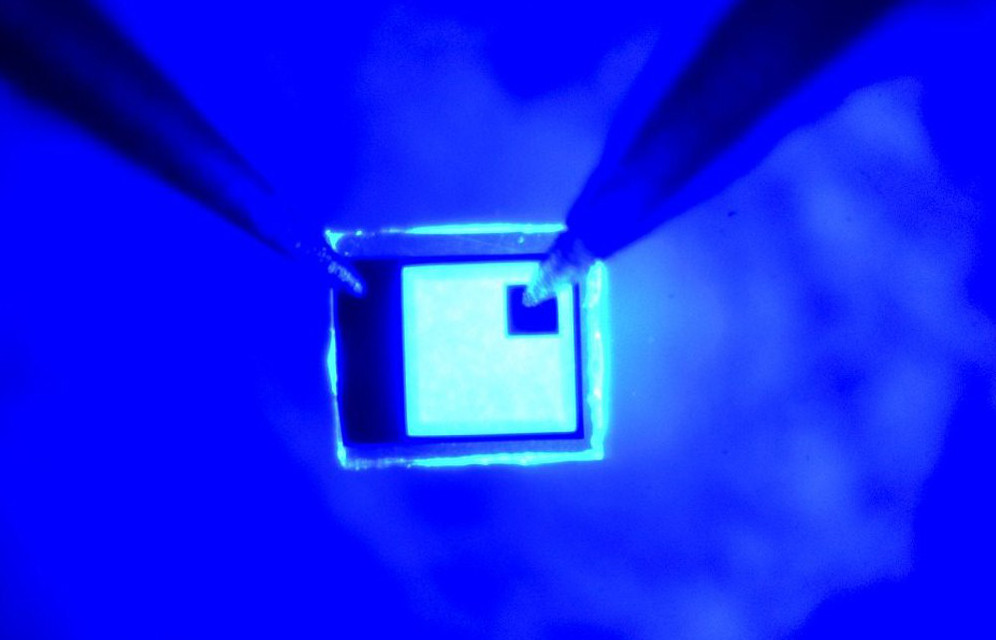
\includegraphics[width=4cm]{./0_intro/img/10-7-14-nobel-prize-blue-led.jpg}
\caption{Picture of a blue LED researched by Shuij Nakamura.}
\label{fig:blue_LED}
%\caption*{Source: \url{http://www.newsweek.com/how-blue-led-changed-world-and-won-nobel-prize-275977} }
\end{figure}

It was not till 1994, with the invention of the high-efficiency blue \emph{light-emitting diode} LED (Fig. \ref{fig:blue_LED}), that the lighting industry had a revolutionary change in the light generation technology. The breakthrough of Shuji Nakamura~\cite{94Nakamura} discovery had such an impact in the last decades that he was awarded with the 2014 Nobel prize in physics. The new LED technology allowed the implement white LEDs with high brightness and settled the bases for the a new player in the lighting market, the \emph{Solid State Lighting} (SSL) industry.
The advantages of SSL are:
\begin{description}
  \item [Efficiency] The light generation inside an LED is produced by the direct mechanism of hold-electron recombination, the supplied energy is a better use of the energy compared to the incandescent lamps. The power consumption can be up to an order of magnitude lower of an incandescent light.

  \item [Size] LEDs are tiny and flat devices, which can be considered as 2-D elements and do not need any vacuum chamber to work. They are much more flexible devices to assembly, and can easily replace the old glass made bulb design.

  \item [Color] LED light has a very narrow light spectrum, that can be used to produce directly colored light. Colored lights are becoming more popular in domestic homes becoming a piece of decoration or mood tweaking device.

  \item [Dynamics] Compared to any of the traditional sources of light LEDs have no dynamics, actually they have but it's very fast and not appreciable to the human eye. Therefore they do not have any setting time when turned on, which is not the case of CFL. The fast dynamics allows to modulate the light and transmit data without disturbing the human beings.

  \item [Lifetime] Solid State devices do not wear off, there fore they can be considered to have an infinite lifetime. In practice LEDs make use of organic phosphores, thus the light quality derates with the use, but the life expectancy of the LED is rated from 20.000 - 100.000 hours, multiplying 20 to 100 times longer that the classical light bulbs.
\end{description}

Such advantages are so relevant that entities like the \emph{United States National Lighting Bureau}~\cite{14USDoE} forecasts a market penetration growth from 5\% in 2015, to the 74\% in 2020 and reaching the 88\% in 2030, as shown in the graph of Figure~\ref{fig:lighting_forecast}. Just with regard to the efficiency, the projected energy savings for 2020 are $297TWh$ only in USA. The \emph{United States Environmental Protection Agency}~\cite{14USDoE} adds that reducing the household lighting energy consumption by half - easy to achieve using with LED lighting -  more than \$13 billion a year in energy costs could be saved, more than 80 million metric $CO_2$ tones would be avoided each year, and the need for over 30 power plants could be eliminated. Therefore these figures make evident that the almost all the lighting technologies will be replaced by LED technology, these movement towards SSL  has been referred as the \emph{LEDification}.

\begin{figure}[!h]
\centering
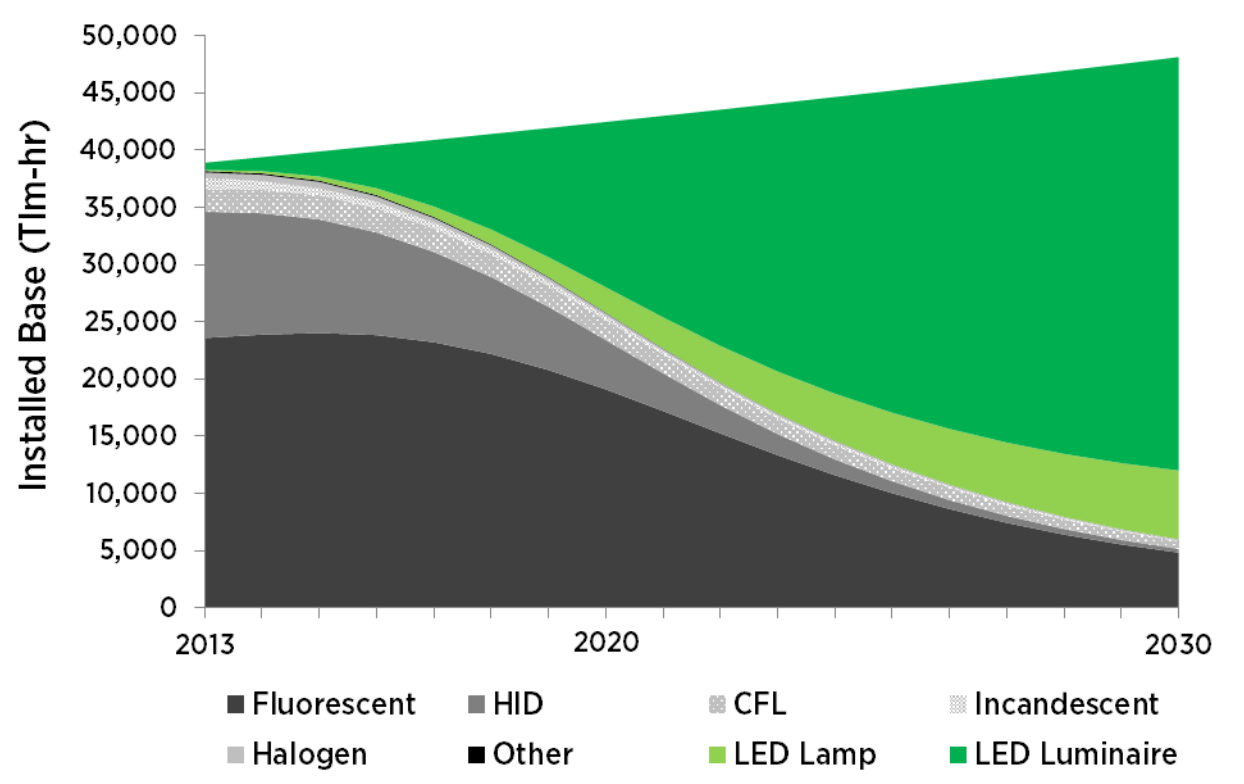
\includegraphics[width=10cm]{./0_intro/img/lighting_forecast.png}
\caption{U.S. Lighting Service Forecast, 2013 to 2030~\cite{14USDoE}.  }
\label{fig:lighting_forecast}
\end{figure}

For the last decade the lighting industry has been in a rush to bring LED light bulbs to the market. First products where putted in the market around 2010, the development has been continuously growing at fast speed making possible that in less than 4 years to find an LED lamp replacement for almost all the incandescent light bulbs.

Today in 2015, LED light bulbs are already available in almost all the lighting ales of the supermarkets and retail shops, however they are not yet adopted as the preferred solution. Despite of the advantages of LED lighting, end consumers are still very reluctant to make the change towards SSL products due to their elevated price. Currently a 100W LED replacement costs between \$20 - \$40 compared to less than \$3 of an halogen incandescent. Actually for consumers is hard to understand that even incandescent are cheaper, LED replacements save money over the life time of the product due to energy savings.

Results in Tab.\ref{tab:lighting_tech} are quite dramatic, looking to the \emph{Lumen cost of owner ship}\footnote{Lumen cost of owner ship is expressed in $klm/$€ indicating how many lumens you can produce per 1€ during thousand hours. Using this metric the different light technologies can be compared independently of the lamp power consumption.} incandescent technologies are below 60 $klm/$€   and LED technology are easily above 200$klm/$€. Translating to total costs\footnote{Lamp amortization are included in the costs}, we could estimate that in a productive year (around 2000$h$) in an office space\footnote{Recommended illumination for productive office spaces is around 500$ lm/m^2 $ } of 20 $ m^2 $ would be above 420€ for incandescent lamps and below 140€ for LED lamps; still linear fluorescent will be the cheapest option with a cost blow 80€ but fluorescence are definitely not suitable for general use. Obviously LED lighting is going to be the future lighting technology, but still the industry has find the manner to initiate the end consumer to buy LED lamps as a first choice.


\begin{landscape}
\thispagestyle{empty}
\begin{table}[h]

\centering
\caption{Characteristics for different lamp technologies (winter 2015).}
\label{tab:lighting_tech}
\renewcommand{\arraystretch}{1.5}% Wider
\begin{tabular}{l | r |  *{10}r }
% after \\: \hline or \cline{col1-col2} \cline{col3-col4} ...
\mcrot{1}{l}{60}{} & \mcrot{1}{c}{0}{Units} & \mcrot{1}{c}{60}{Incandescent}  & \mcrot{1}{c}{60}{Halogen} &  \mcrot{1}{c}{60}{Cold-White Fluorescent} & \mcrot{1}{c}{60}{Warm-White Fluorescent}& \mcrot{1}{c}{60}{Compact Fluorescent} & \mcrot{1}{c}{60}{HDI SON} & \mcrot{1}{c}{60}{Retrofit LED Budget } & \mcrot{1}{c}{60}{Retrofit LED Dimmable } & \mcrot{1}{c}{60}{Retrofit LED} & \mcrot{1}{c}{60}{Retrofit Tube LED}  \\
  \midrule

  Power                     & $W$            & 100   & 53    & 36    & 39    & 11    & 70    & 10    & 13    &  5  & 10.5  \\
  Flux                      & $lm$           & 1203  & 845   & 3100  & 3100  & 600   & 5600  & 600   & 1055  &   350  & 950   \\
  Efficacy                  & $lm/W$         & 14.3  & 14.42 & 57.14 & 57.14 & 55    & 80    & 60    & 81.15 &    70  & 90.5  \\
  Color Temperature         & $K$            & 2700  & 2800  & 4000  &  3000 & 2700  & 2000  & 2700  & 2700  &  3000  & 3000  \\
  Color Rendering Index     &                & 100   & 100   &   85  &  85   &  82   &  25   & 87    & 80    &  80    & 85    \\
  Lifespan                  & $h$            & 1000  & 2000  & 20000 & 24000 & 15000 & 28000 & 2500  & 25000 & 15000  & 50000 \\
  Retail price              & €          & 1     & 3     & 5.6   & 4.8   & 8.78  & 14.26 & 4.5   & 37.1  & 17     & 43    \\
  Lumen cost of ownership   & $ klmh/$€ & 48    &   59  & 348   & 324   & 186   & 324   & 233    & 229   &  182   & 281   \\
  Cost of ownership         & €$/kh$     & 25    &  14.2 & 8.9  & 9.6   & 3.2   &  17.3 & 2.6    &  4.6  &  3.3   & 3.4   \\
  Cost for a 20$m^2$ office & €$/kh$     & 260    & 210 & 36     & 39    & 67     & 39  &  54   &  55    & 69     & 43 \\
%  \hline
\end{tabular}
\end{table}
\end{landscape}

\vspace{5mm} %5mm vertical space


\begin{figure}[!h]
\centering
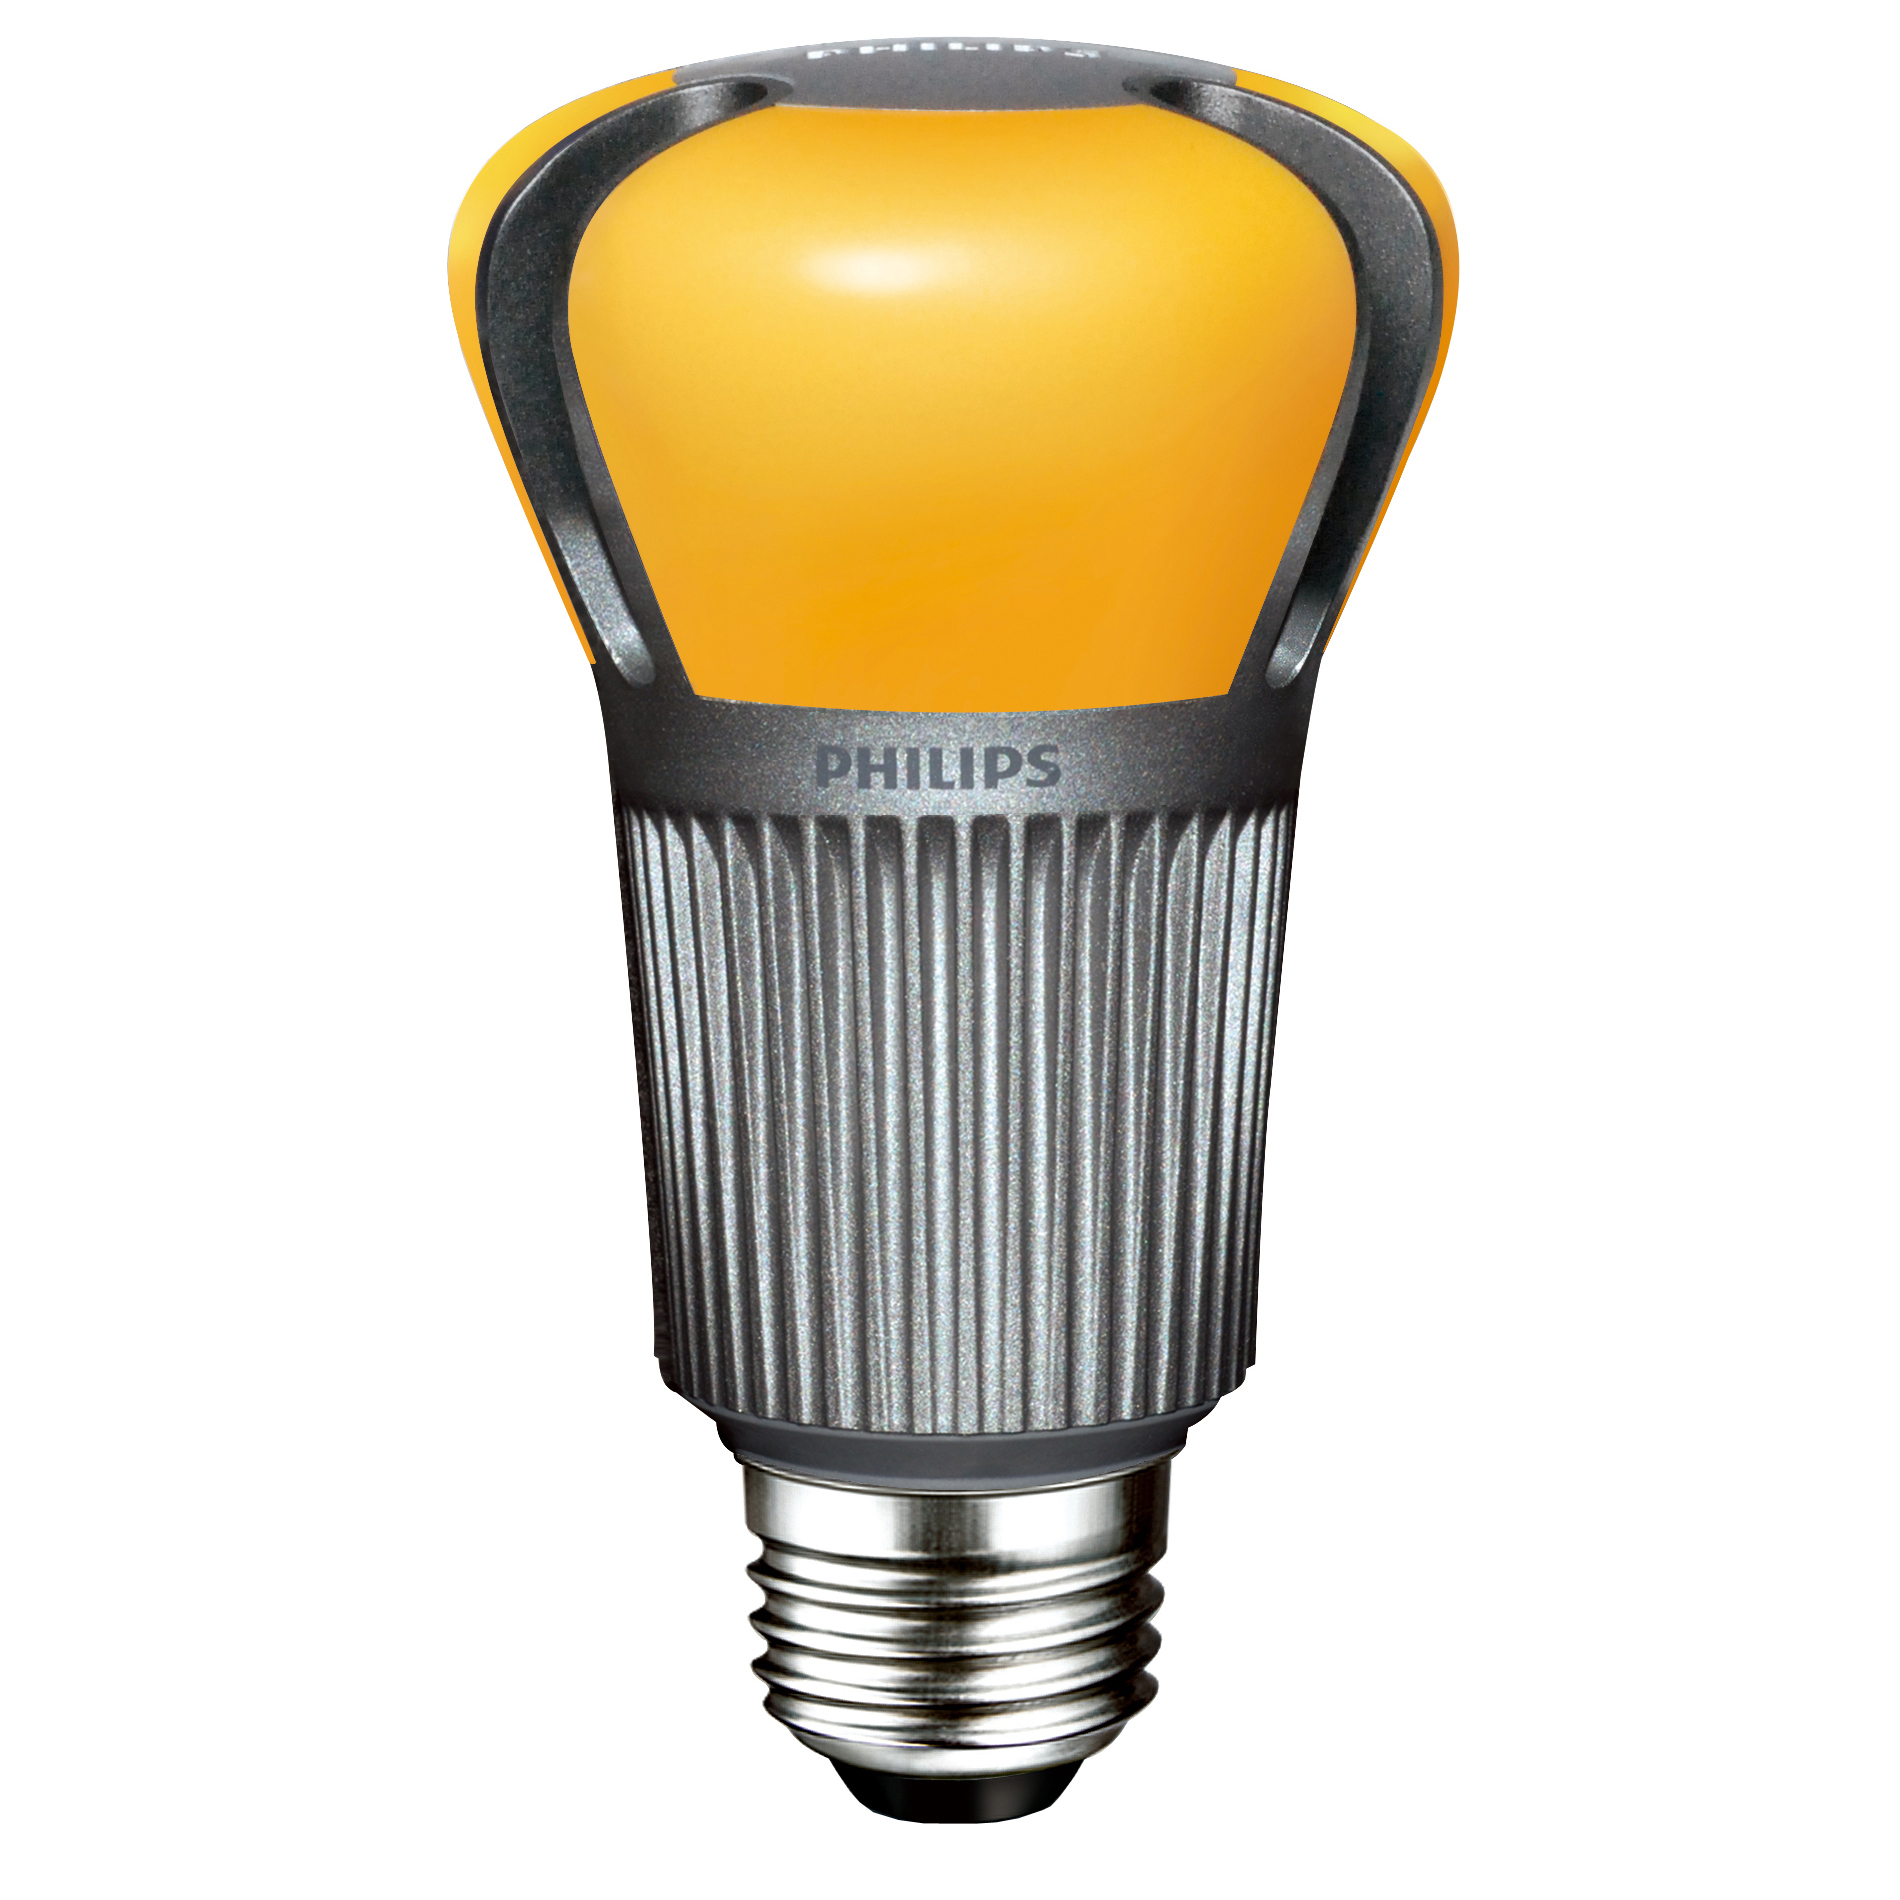
\includegraphics[width=4cm]{./0_intro/img/enduraled-12w.jpg}
\caption{900 lumens LED light bulb.}
\label{fig:l_prize}
\end{figure}

Different factors can help the adoption of the SSL as the preferred lighting solution in the market. On the one hand reducing the end product price, and on the other hand, bringing more value to the traditional lighting sources. Actually LED light bulbs already bring more value compared to the old light bulbs being much more efficient, almost one order of magnitude lower in power consumption, and a longer lifetime, easily twenty times more operating hours. However these factors are not yet a valuable argument for the consumers. Other advantages that LED lamps are starting to offer are color tuning, light level dimming, smart-phone control and wireless services; positioning SSL in line with the current trend of the \emph{internet-of-things} for lighting \emph{internet-of-lights}. Moreover, LED lighting is also growing the luminaires industry, being more and more popular the LED luminaries where the luminaries already incorporate the LEDs without using lamps and taking advantage of the design possibilities that allow the small form facto of the LEDs, as a matter of fact the \emph{U.S Department of Energy} (U.S.DoE) estimate that LED luminaries will be the big player in the lighting market as shown in Fig.\ref{fig:lighting_forecast}.

Overall we can identify three main factors that influence in the market penetration of SSL:
\begin{itemize}
  \item Price
  \item Intelligence: Interactivity, connectivity and controllability\
  \item Light fixture size: Luminaire design, shape and application
\end{itemize}

In order to relate the aforementioned factors in the development of a LED light system and understand the challenges is essential to describe the different elements that compose an LED light. A LED light system is composed by the six main elements described below and shown in  the Figure~\ref{fig:exploded_bulb}.

\begin{description}
  \item[LED] A two-lead semiconductor device that produced light when a current flows through it and its name comes form the acronym \emph{Light-Emitting Diode}. Internally light is produced by the electroluminescence effect, when an electron recombines with an electron-hole releasing energy in form of photons. The color of the light is determined by the energy band gap of the semiconductor.

      The selection of the LEDs will determine the light color, load characteristics, power, efficiency and the load characteristics.

  \item[Optics] Optical device that mixes and distributes the light from the LED to the illuminated space.

  \item[Driver] Electronic circuit designed to transform the electrical power of the input source to properly supply the LEDs. LED drivers are considered current-to-voltage (V-I) power supplies, since almost all the common power supplies are voltage sources and LEDs need to be supplied by current.

      The driver controls the current thought the load, hence the light output, and it is the active part of the system where the control of the lamp relies.

  \item[Heat sink] Mechanical element that acts as a passive heat exchanger to cool the hot elements inside the lamp by dissipating the heat into the surrounding medium. In the LED system the energy that is not transformed to light becomes heat and must be extracted from the lamp. The hot spots areas in the lamp are localized at the LEDs chips and at the driver components.

  \item[Body assembly] Mechanical element that hold all the different subsystems in one single device. In many cases the heat sink does this functionality.

  \item[Connector] Mechanical element that provides connection with the energy source. The most popular one is the Edison connector present in all screw-in lamps. There are many other popular ones such as GU10, MR16, MR11 coming from the halogen multifaceted reflector bulbs or the 2-pin connector of the fluorescent tubes.

      In many cases, the standardized connectors suppose a restriction for the mechanical design of the lamp. Their old-fashioned design is not optimal for the new lamps.
\end{description}

Now, with a better understanding of the elements of a LED lamp we can relate them to the three factors that influence the market penetration. First the price, the Figure~\ref{fig:cost_breakdown} shows the cost breakdown for different lighting applications, it can be seen that the LED costs are more or less distributed between Driver, LED package and Thermal/Mechanical/Electrical, comprising this last group the heat sink, the connector socket and the \emph{Printed circuit Board} (PCB) that interconnects input socket, LEDs and driver. As shown in Figure~\ref{fig:cost_breakdown_forecast} the cost distribution is predicted to keep similar being even a bit better distributed among this three players. That is why research efforts regarding cost down are being played all for all the different subsystems in the lamp in order to fulfill the predicted total cost reduction of one half from now till 2020.  

%\begin{figure}[!h]
%\centering
%\begin{subfigure}[t]{.45\textwidth}
% % \centering
%  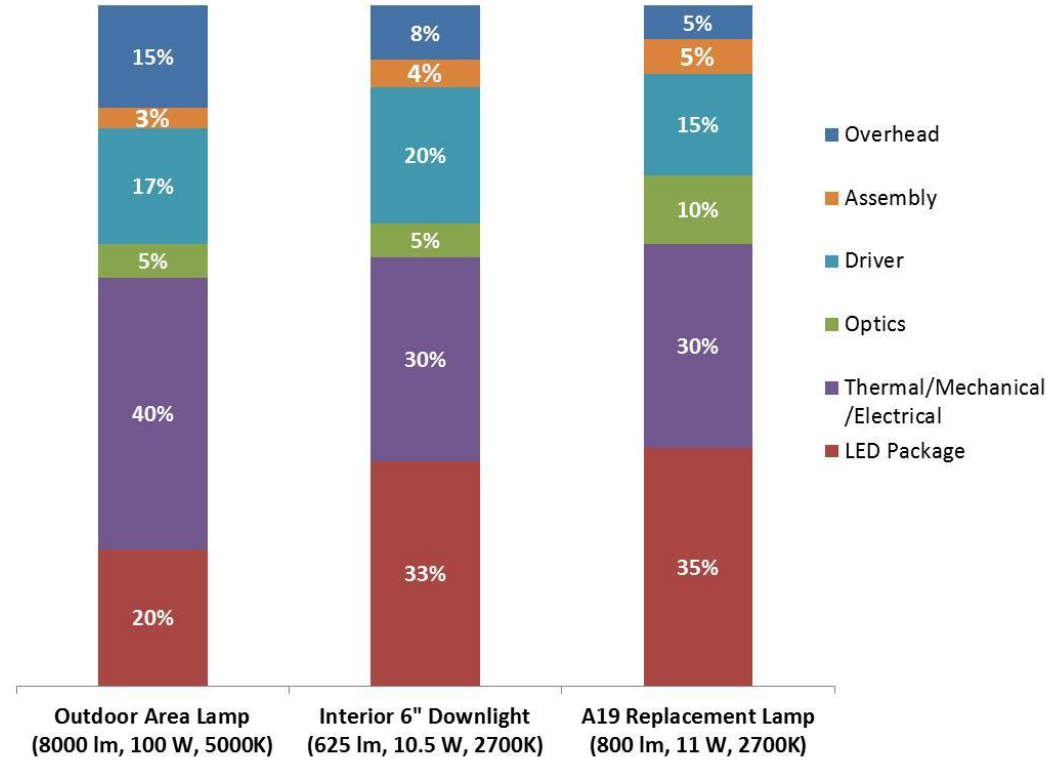
\includegraphics[width=\textwidth]{./0_intro/img/cost_breakdown.png}
%  \caption{}
%  \label{fig:cost_breakdown}
%\end{subfigure}
%
%\begin{subfigure}[t]{.45\textwidth}
%  %\centering
%  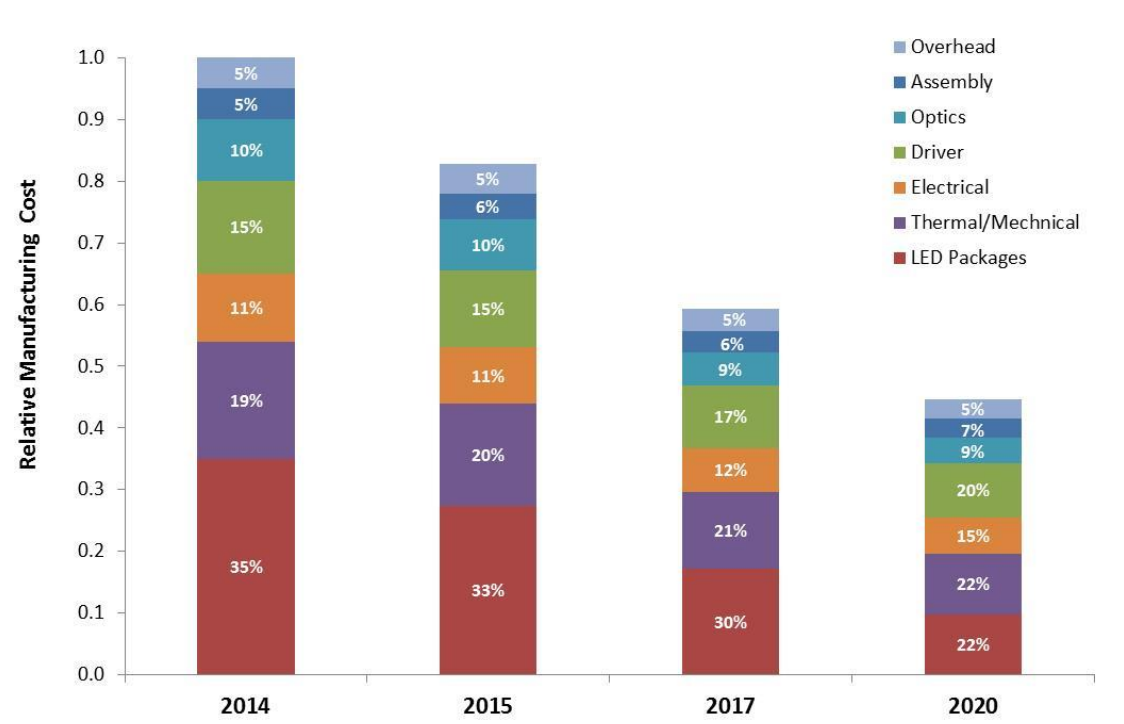
\includegraphics[width=\textwidth]{./0_intro/img/cost_breakdown_forecast.png}
%  %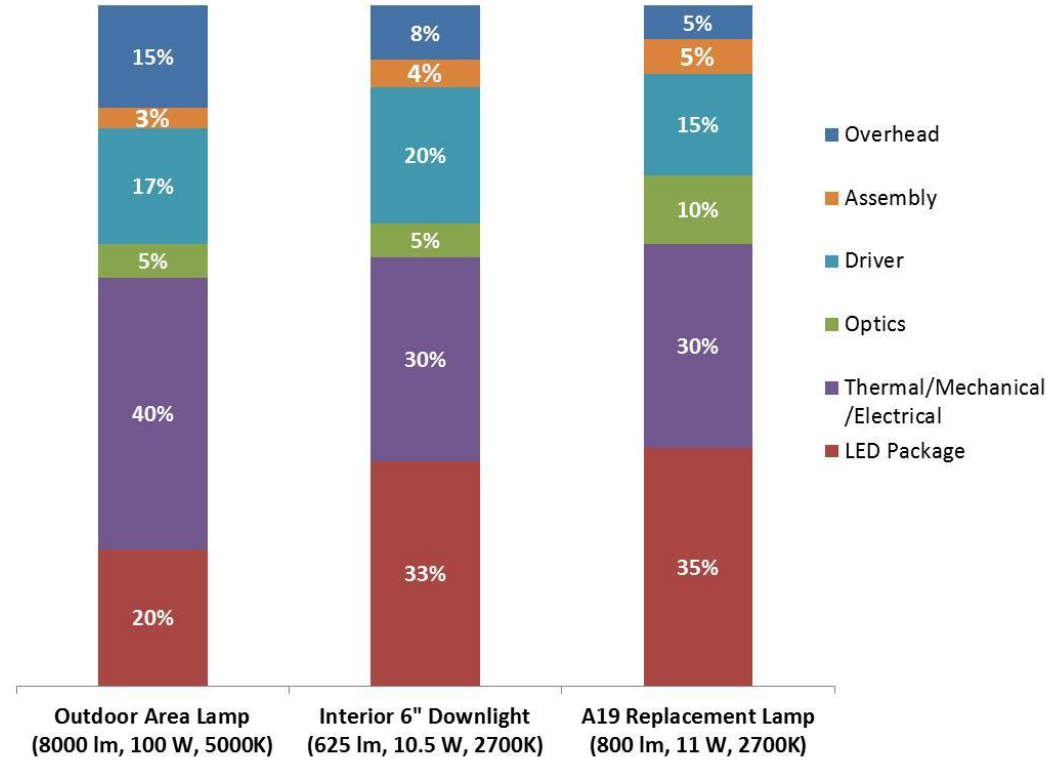
\includegraphics[width=\textwidth]{./0_intro/img/cost_breakdown.png}
%  \caption{}
%  \label{fig:cost_breakdown_forecast}
%\end{subfigure}
%\caption{\emph{Source: DOE SSL Roundtable and Workshop attendees}}
%\label{fig:costs_BD_FC}
%\end{figure}

\begin{figure}[!h]
\centering
\subcaptionbox{\label{fig:cost_breakdown}}[0.5\textwidth]
   {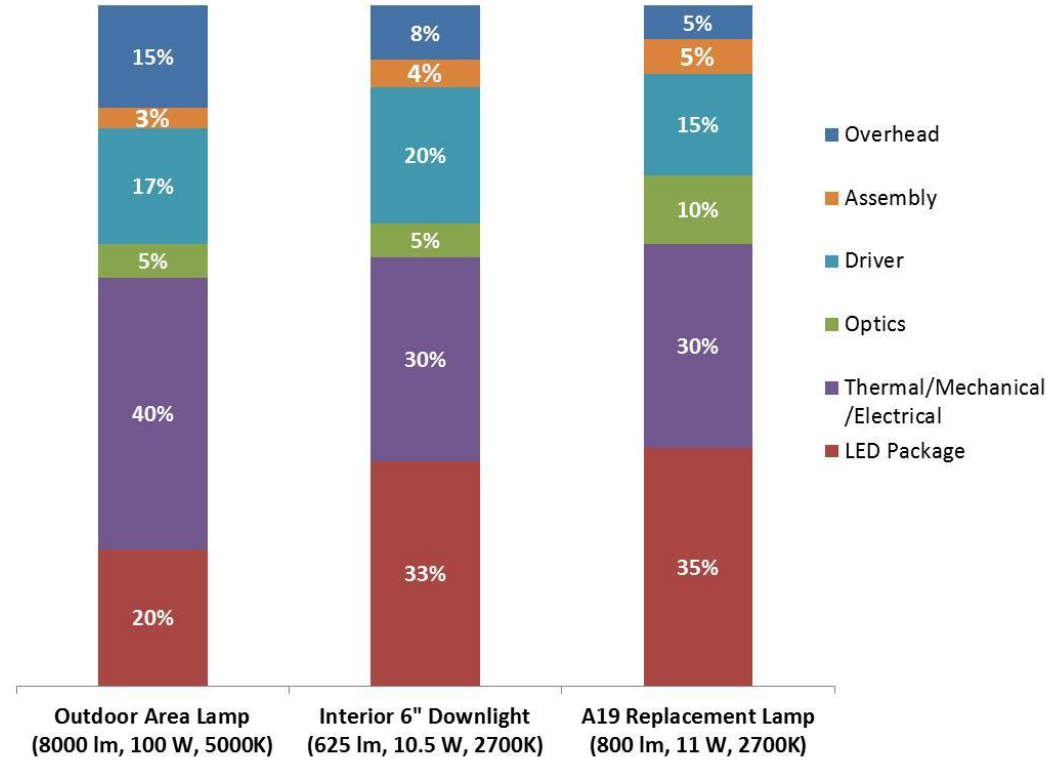
\includegraphics[width=0.45\textwidth]{./0_intro/img/cost_breakdown.png}}

\subcaptionbox{\label{fig:cost_breakdown_forecast}}[0.5\textwidth]
   {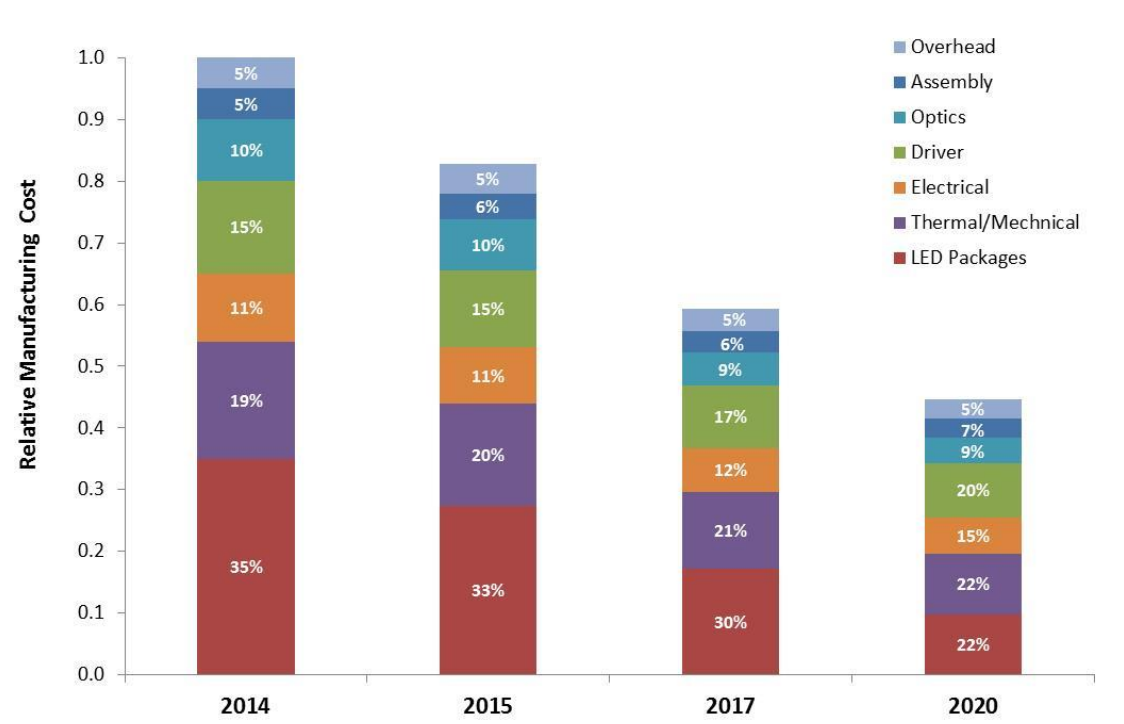
\includegraphics[width=0.45\textwidth]{./0_intro/img/cost_breakdown_forecast.png}}
\caption{\emph{Source: DOE SSL Roundtable and Workshop attendees}}
\label{fig:costs_BD_FC}
\end{figure}

The other two aspects functionality and lamp size can be narrowed down to a single element in the lamp system: The Driver. On the one hand the driver is the only element that brings the functionality to the lamp, therefore the only one that can incorporate the control and interactivity to the system. On the other hand, it also influences the design of the lamp. Since the driver controls the LEDs the closer the driver to the LEDs is the better for the entire system, being this is one of the design restrictions that plays the driver. The large volume of some components of the driver restrict to take advantage of the low from factor of the LEDs.   


\begin{figure}[!h]
    \centering
    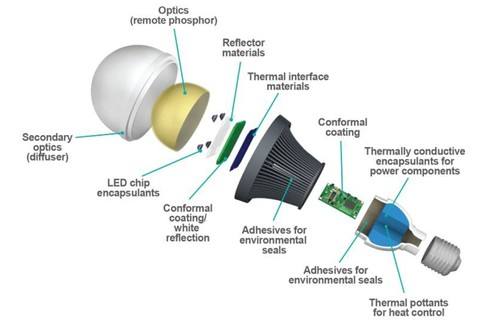
\includegraphics[width=8cm]{./0_intro/img/exploded_bulb_2.jpg}
    \caption{Exploded vision of an LED light bulb.}
    \label{fig:exploded_bulb}
\end{figure}


Reducing the costs of the lamps has been the strategy taken for the first wave in the \emph{LEDification} process where retrofitting\footnote{Adding the new LED technology to the older light bulb systems. In that way the end user can directly replace an incandescent lamp or a florescent tub by an LED one without needing to make any change in the current installation.} the old lamps is chosen as the way to target the end costumer. In on the one hand, fruitful results came form that research with new innovative solutions at very low costs that could be packed in almost all the light bulb shapes currently commercially available. But in the other hand, these new drivers had the incontinent of using very old components that at the same time restricted reduction of the circuit volume and made more complex the addition of extra control functionalities while keeping the initial low costs.

\begin{figure}[!h]
\centering
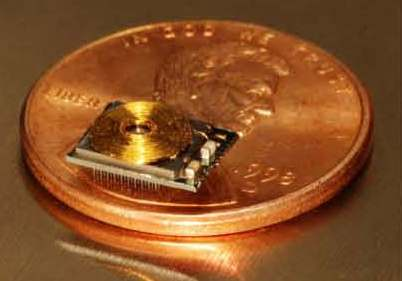
\includegraphics[width=8cm]{./0_intro/img/FSolzbacher01.jpg}
\caption{Power System in a Package die. The circuit implements a buck converter.}
\label{fig:psoc_example}
\end{figure}

\vspace{5mm} %5mm vertical space

The second line of research has focus on reducing the volume of the driver circuit. That research topic arose when comparing the the volume of the LEDs and the driver, it is evidenced a mismatch between the two volume of the components, becoming in many cases the driver circuit the dominant element of the entire lamp. Such mechanical constrain supposes an obstacle to take the full advantage of the low form-facto of the LED in the future luminaries, where LED will not be assembled using the old fashioned cases. Therefore, that research has a much longer term vision for targeting the second of third generation of lights in the \emph{LEDification} process.

The drive to reduce the volume of the drivers led to focus the research from the perspective of the integrated power supplies, where the power converter can be partially or fully integrated in a single package. There are two approaches of integrated power converters: \emph{Power System on Chip} (PSoC) or  \emph{Power System in Package} (PSiP). The first integrate all required power components, active and passive, in a single die. The second assemble all the components within the same package, keeping the appearance of an unique \emph{Integrated Circuit} (IC), see Figure~\ref{fig:psoc_example}. The advantages of having an integrated power management unit align with the necessities of the LED drivers, therefore trend of the drivers will be going towards having \emph{Power LED Drivers in Package} (PLDiP).

Besides the size reduction that an integrated driver would suppose, an integrated approach would also bring other benefits in terms of control and connectivity. Since such a solution would require a the design of a dedicated \emph{application-specific integrated circuit} (ASIC), the power management unit and driver control unit can be integrated together, providing the necessary intelligence for light control and the connectivity optimized for the requirements of the coming connected lighting industry. The \emph{Philips} \emph{HUE} lamp is a clear example of the requirements of the so called \emph{smart drivers}. That lamp provides a full light color gamut color control through a mobile and web application or through a remote control. The internal driver has four light channels red, green, orange and additional amber and at the same time provides wireless connectivity through ZigBee, being the electronic board populated with discrete power drivers and few micro-controller units. A solution that integrates all the functions in a single IC, or few ICs (one per channel), will definitely reduce packaging and assembling costs and still providing the same functionalities. And at the same time, the expected market size for LED lighting to justify a dedicated ASIC design for the light bulbs and indeed has been the motivation of this thesis. Therefore goal of this work was to explore and identify new architectures that are suitable for integration and at the same time can perform as an efficient LED driver.


\section{Why a LED needs a driver?}

As shown in Figure~\ref{fig:led_I-V} a LED has a very abrupt V-I curve. For voltages below the \emph{forward voltage}, $V_{f}$, there is no current flow and the LED behaves as an open circuit. For voltages above $V_{f}$ the curve becomes very steep and the current increases dramatically with respect to the voltages, thus the LED behaves as short circuit. The driver bias the LED to a specific point, $P$ in Figure~\ref{fig:led_I-V}, providing the desired output light. The colour and flux (light intensity) will vary depending of the bias point.  Since the majority of  available  energy sources are  voltage sources, and LED requires a circuit that limits the current that flows through it, that circuit is the LED driver.

\begin{figure}[!h]
\centering
\begin{tikzpicture}[domain=0:5]
    \draw [->] (0,0) -- (4.5,0) node[anchor=west]{$V$};
    \draw [->] (0,0) -- (0,4.5) node[anchor=east]{$I$};

    %Mark Vth
    \draw (2,2pt) -- (2,-5pt) node[anchor=north] {$V_{f}$};

    %Draw ideal plot
    \draw[thick] (0,0) -- (2,0) -- (4,4);

    %Draw bias points
    \draw[dashed] (3,2) -- (3,-0);
    \draw (3,2pt) -- (3,-5pt) node[anchor=north]  {$V_{bias}$};

    \draw[dashed] (3,2) -- (-0,2);
    \draw (2pt,2) -- (-5pt,2) node[anchor=east]  {$I_{bias}$};
    \filldraw (3,2) circle(2pt) node[anchor=west] {$P$};



\end{tikzpicture}
\caption {}
\label{fig:led_I-V}
\end{figure}

At the first glance, keeping a constant bias current, $I_bias$, through the LED does not seems to be challenging. However LED V-I characteristic is not static, in practice LEDs has different source of deviations and drivers have to deal with them in order to keep delivering the desired light output. First, $V_f$ has a negative dependence with the temperature, drooping its values as the PN junction temperature increases. Second, the LED has an aging factor derating its light output over time, which has to be adjusted by changing the bias point. And last but not least, during production LEDs will vary in colour, flux and forward voltage; even for products from the same batch. The manufacturer reduced the dispersion between devices by binning \footnote{Quality control performed at LED production line, where each LED is individual tested and sorted in groups (bins) that have the same electrical and lighting characteristics.}, but still after binning it can be deviations from up to $10\%$ in $V_f$ for the same part number.

Up to date, there are three big families of LED drivers that will be presented in the following sections.

\section{Linear Drivers}

 Linear drivers place a shunt element between the source and the LED. The shunt element limits the current in the LED providing the necessary voltage droop between the source and the load. The excess of voltage between the source and the load is dissipated in the shunt element, literally burned in form of heat; therefore this drivers become very inefficient if the LED voltage is not close to the source. Moreover this drivers can only provide step-down conversion, thus they cannot work when the load voltage is higher than the input supply.

\begin{figure}[!h]
        \centering
        \ctikzset { bipoles/length=1cm}
        \begin{circuitikz} [scale=0.65]
        \draw
        (5,0) to[short]
        (0,0) to[V = $v_{src}$]
        (0,3) to[generic=${Shunt}$,i=$i_o$]
        (5,3);
        \draw
        (5,0) to[leD*,v_>=$v_{o}$] (5,3);

        \begin{scope}[xshift = 8cm, yshift=0cm]
            \draw[->] (0,0) -- (4,0) node[anchor=north] {$  m $};
            \draw[->] (0,0) -- (0,3.2) node[anchor=east] {$\eta $};

            %Ticks X
            \draw (3,2pt) -- (3,-5pt) node[anchor=north] {$1$};
            \draw (1.5,2pt) -- (1.5,-5pt) node[anchor=north] {$0.7$};

            %Ticks Y
            \draw (2pt,2.5) -- (-5pt,2.5) node[anchor=east] {$100\%$};
            \draw (2pt,1.5) -- (-5pt,1.5) node[anchor=east] {$70\%$};

            %Markers
            \draw[dotted] (3,2.5) -- (3,0);
            \draw[dotted] (3,2.5) -- (0,2.5);
            \draw[dotted] (1.5,1.5) -- (1.5,0);
            \draw[dotted] (1.5,1.5) -- (0,1.5);


            \draw[thick] (3,2.5) -- (0,0.5);



        \end{scope}

        \end{circuitikz}
        \caption{Linear LED driver schematic}
        \label{fig:linear_drv}
       \end{figure}

   The circuit of the Figure~\ref{fig:linear_drv} shows schematic of a linear driver, the shunt element can be implemented with just a resister of with an active device, the second enables regulation for variations in the source and in the load. Both cases linear drivers are very simple to implement, with very low costs and taking almost no volume, being indeed the perfect solution for integration.



   The plotted graph presents the variation of the driver efficiency with respect to the conversion ration $m$. $m$  is the ratio between the input voltage, $v_{src}$,  and the output voltage,$v_o$, being defined as
   \begin{equation}
        m = \frac{v_o}{v_{src}}.
   \end{equation}

   The efficiency of the driver is the ratio between the input power and the output power
   \begin{equation}
        \eta = \frac{P_o}{P_i} = \frac{v_o i_o}{v_{src} i_o} = \frac{v_o}{v_{src}},
   \end{equation}
   thus we can see that for this case the efficiency is indeed the conversion ratio
   \begin{equation}
        \eta = m,
   \end{equation}
   owing to the fact that LED drivers have to be efficient, saying that at worst case 80\% efficiency can be accepted, such drivers could only be suitable where the ration between input voltage and load voltage is 0.8.

   Despite the fact that linear drivers are cheap and easy to integrate, their poor efficiencies and limitations in power conversion palace them in a unfavorable position as a realistic sortition for an integrated solution.

\section{Inductor Based Converters}

Inductor Based Converters (IBCs) are \emph{Switched Mode Power Supplies} (SMPS) \footnote{Electronic power supply that provides efficient electric power conversion by commuting between different circuit configurations (modes).}  that employ magnetic passive elements (i.e. inductors and transformers) to store energy and provide efficient electrical power conversion. Since IBCs have are very efficient in voltage-to-current conversion they are ideal as LED drivers.

This converters can provide step-up and step-down conversion for large dynamic ranges while keeping the efficiency very high. Besides the power conversion capabilities, these converters can provide also galvanic isolation, which, in many application, is compulsory in order to guarantee the safety of the users against electrical hazards. Such characteristics place these drivers as the preferred solution for the LED drivers manufacturers. Figure~\ref{fig:inductive_smps} the regulation characteristic curve of an inductor based converter. As shown, the theoretical efficiency of these converters is 100\% among all the conversion ratio range, in practice due to the parasitics in switches and inductors, the efficiency drops to a certain value with small fluctuations with respect to the conversion range.

Despite the aforementioned advantages of these converters they are not still very bulky with respect to the LEDs.  In practice, inductors dominate the entire volume of the LED drivers as shown in Figure~\ref{fig:smps_driver}.

\begin{figure}[!h]
      \centering
\ctikzset { bipoles/length=1cm}
\begin{circuitikz}[scale=0.65]
\draw
    (2.5,0) to[short]
    (0,0) to[V = $V_{src}$]
    (0,3) to[short]
    (2.5,3) ;

\draw
    (2,3) --
    (2.5,3)

    (2,0) --
    (2.5,0)

    node  (IC)  at (2,0) {}
    node  (I) at (2,3) {}
    (I) to[open,v=$v_{i}$] (IC);


\draw [thick]
    (2.5,-0.5) --
    (2.5,3.5)  --
    (5.5,3.5)  --
    (5.5,-0.5) --
    (2.5,-0.5);

\draw (4,3.25)node[anchor=north]{$\frac{v_o}{v_{i}}=m$} ;

\draw (3.5,2) to[L] (3.5,0);
\draw (4.5,2) to[switch] (4.5,0);


\draw
    (5.5,0) to[short]
    (7,0) to[ leD*,v_>=$v_{o}$]
    (7,3) to[short,i_<=$i_o$]
    (5.5,3) ;


\begin{scope}[xshift = 10cm, yshift=0cm]
            \draw[->] (0,0) -- (4,0) node[anchor=north] {$  m $};
            \draw[->] (0,0) -- (0,3.2) node[anchor=east] {$\eta $};

            %Ticks X
            %\draw (3,2pt) -- (3,-5pt) node[anchor=north] {$1$};
            %\draw (1.5,2pt) -- (1.5,-5pt) node[anchor=north] {$0.7$};

            %Ticks Y
            \draw (2pt,2.5) -- (-5pt,2.5) node[anchor=east] {$100\%$};
            \draw (2pt,1.5) -- (-5pt,1.5) node[anchor=east] {$90\%$};

            %Markers
           % \draw[dotted] (3,2.5) -- (3,0);
            \draw[dotted] (3,2.5) -- (0,2.5);
            %\draw[dotted] (1.5,1.5) -- (1.5,0);
            \draw[dotted] (1.5,1.5) -- (0,1.5);


            \draw[thick] (0.5,2.5) -- (3,2.5) node[anchor=south] {$Theoretical$};
            \draw[thick,dashed] (0.5,1.20) parabola[bend at end] (3,1.7) node[anchor=north] {$Real$};
        \end{scope}
\end{circuitikz}
\caption{Generic two port block diagram of an inductor based SMPS, and the regulation-efficacy characteristic comparing the \emph{Theoretical} limit and the \emph{Real} case. }
\label{fig:inductive_smps}
\end{figure}


Increasing the switching frequency or reducing the voltages swing are the two possible methods in order to reduce the value, thus the size, of the magnetic components.

Miniaturization of magnetic components is a challenge due to of their 3-D mechanical structure.
The performances of the integrated inductors are still far to fulfil the requirements for the consumer applications.  Research in that field are presenting new structures that can be assembled in the same package with the active devices, but the switching frequencies of the discrete derivers is not high enough to make use them.

\begin{figure}[!h]
\centering
\begin{tikzpicture}
\node[anchor=south west,inner sep=0] (image) at (0,0) {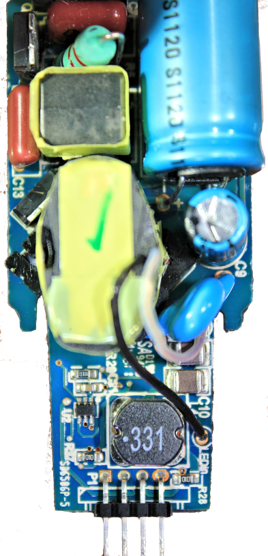
\includegraphics[height=5cm,angle=90]{./0_intro/img/LED_driver.png}};
\begin{scope}[x={(image.south east)},y={(image.north west)}]
\draw[red,ultra thick,rounded corners] (0.70,0.3805) rectangle (0.855,0.7);
\draw[red,ultra thick,rounded corners] (0.11,0.1) rectangle (0.28,0.50);
\draw[red,ultra thick,rounded corners] (0.28,0.1) rectangle (0.63,0.62);
\end{scope}
\end{tikzpicture}
\caption{Magnetic components marked with a red square in a mains connected LED driver. The magnetic components dominate the volume of the converter.}
\label{fig:smps_driver}
\end{figure}






\section{Switched Capacitors}
Switched Capacitor Converters (SCCs) are \emph{dc-dc} power circuits composed only by switches and capacitors that provide efficient voltage conversion. SCCs have been long known and utilized, initially for voltage multiplication and more recently for voltage regulation as well. Compared to inductor based power converters, the absence of magnetic elements makes them suitable for high density power systems and integrated solutions , such as Power-System-in-Package (PSiP) or Power-System-on-Chip (PSoC).

SCCs have a fix ratio of conversion between the input and the output determined by the topology. The output voltage of the converter under no load conditions is defined as \emph{target voltage} ($v_t$), and its efficiency is very high when the load is supplied close to the \emph{target voltage}. If the output voltage goes below the \emph{target voltage} the efficiency drops, similar to the linear drivers.  The converter can not supply voltages above the \emph{target voltage}.

A common practice to extend the regulation margins of these converters is to have topologies with multiple conversion rations as shown in the plot of Figure~\ref{fig:SCC_driver}. We can see that efficiency increases as the ration $m$ gets close to the first fixed conversion ration of the converter $m_1$; right after $m_1$ the efficiency drops dramatically and it linearly increases as it approaches the second fixed conversion ratio of the converter $m_2$.

\begin{figure}[!h]
      \centering
\ctikzset { bipoles/length=1cm}
\begin{circuitikz}[scale=0.65]
\draw
    (2.5,0) to[short]
    (0,0) to[V = $V_{src}$]
    (0,3) to[short]
    (2.5,3) ;

\draw
    (2,3) --
    (2.5,3)

    (2,0) --
    (2.5,0)

    node  (IC)  at (2,0) {}
    node  (I) at (2,3) {}
    (I) to[open,v=$v_{i}$] (IC);


\draw [thick]
    (2.5,-0.5) --
    (2.5,3.5)  --
    (5.5,3.5)  --
    (5.5,-0.5) --
    (2.5,-0.5);

\draw (4,3.25)node[anchor=north]{$\frac{v_o}{v_{i}}=m$} ;

\draw (3.5,2) to[C] (3.5,0);
\draw (4.5,2) to[switch] (4.5,0);


\draw
    (5.5,0) to[short]
    (7,0) to[ leD*,v_>=$v_{o}$]
    (7,3) to[short,i_<=$i_o$]
    (5.5,3) ;


\begin{scope}[xshift = 10cm, yshift=0cm]
            \draw[->] (0,0) -- (4,0) node[anchor=north] {$  m $};
            \draw[->] (0,0) -- (0,3.2) node[anchor=east] {$\eta $};

            %Ticks X
            \draw (1.75,2pt) -- (1.75,-5pt) node[anchor=north] {$m_1$};
            \draw (3,2pt) -- (3,-5pt) node[anchor=north] {$m_2$};
            %\draw (1.5,2pt) -- (1.5,-5pt) node[anchor=north] {$0.7$};

            %Ticks Y
            \draw (2pt,2.5) -- (-5pt,2.5) node[anchor=east] {$100\%$};
            \draw (2pt,1.5) -- (-5pt,1.5) node[anchor=east] {$90\%$};

            %Markers
            \draw[dotted] (1.75,2.4) -- (1.75,0);
            \draw[dotted] (3,2.3) -- (3,0);
            \draw[dotted] (3,2.5) -- (0,2.5);
            %\draw[dotted] (1.5,1.5) -- (1.5,0);
            %\draw[dotted] (1.5,1.5) -- (0,1.5);


            \draw[thick] (0.5,1.4) -- (1.75,2.4) -- (1.75,1.6) -- (3,2.3)  node[anchor=south] {};
            %\draw[thick,dashed] (0.5,1.20) parabola[bend at end] (3,1.7)[anchor=north] {};
        \end{scope}
  \end{circuitikz}
\caption{Generic two port block diagram of an inductor based SMPS, and the regulation-efficacy characteristic comparing the \emph{Theoretical} limit and the \emph{Real} case. }
\label{fig:inductive_smps}
\end{figure}

The main advantages of these converters is that they use no inductors, which make them very favorable for integration. Integrated capacitors have a better energy density than integrated inductors. The mechanical structure of the capacitors, a stack of isolator-metal-isolator, is much easier to replicate in small scale.
Other advantage of the switch capacitors is that they divide the absolute voltage applied to the converter with the different elements, thus reducing the voltage stress in the switches and capacitors. This voltage reduction in the components is also very relevant from the point of view of integration. First, at lower voltage capacitors have better performances: more energy density, less derating and better chances of integration. Second, lower voltage switches perform better at high frequencies. And third, the lower the blocking voltage of switches is the less silicon area needed and the more standard the fabrication process is, thus reducing the production costs.

The big disadvantage of these converters is that they can not provide voltage-to-current conversion. Nevertheless, they are used for as LED driver in backlighting applications for battery supplied portable devices. In such cases, the SCCs steps-up or steps-down the battery voltage and afterwards a linear driver   provides the tight regulation that LEDs require. Adopting that architecture for general lighting could be a solution, but when we scale voltages and currents to the values used in such applications,  the number of necessary conversion steps of the SCC would make it totally infeasible and inefficient.

On the one hand, the limitation in voltage-to-current conversion would place switched capacitors out of the target architectures as power LED drivers circuits. But on the other hand, their advantageous characteristics for integration made this circuits very attractive as a possible solution for an PSoC/PSiP LED driver. Both arguments have been the motivation and the driver of the research presented in this book.

The book is divided in the four main sections that where necessary to build a switched capacitor LED driver. The first section introduces the new LED driver architecture used during the entire thesis, the \emph{Hybrid-Switched Capacitor Converter}, H-SCC from now on. The second part of this book, the core of this dissertation, presents the methodology to model H-SCC. The methodology extends the previous works in the topic providing an enhanced modeling for the design of SCCs and H-SCCs. The third section is devoted to the practical use of the new methodology, thus for the design phase of a converter. The modeling is used  to help in the development facilitating the sizing and optimization of the design variables. The last section presents a discrete implementation of 12W H-SCC LED driver and the design procedure. Although is not a regular practice, experimental work is not only presented in the in the last section. The experimental work has been used to also validate the new modeling methodology. The final section is the conclusion of the entire work and the new opportunities that can follow from it.


